\subsection{The Nodes and their Managers [Herbert]}
\label{sec:Compiler.Core.NodesAndManagers}
INSPIRE, the Insieme IR, is a formal language designed for modeling all aspects
of a program using a compact, uniform representation. This covers types,
statement and functions as well as expressions (=values).

\subsubsection{An Overview}
An essential obligation of the compiler core is to provide the data structure
required for representing IR codes within a C++ application. Due to the
hierarchical structure of INSPIRE, every code fragment can be modeled as a
simple tree -- where each node has a type and a (potentially) variable length
child list. However, implementing such a representation in a straight-forward
way would require a large number of redundant sub-trees since. For instance,
frequently used IR trees like the one representing the simple integer type --
which due to modeling reasons require at least 3 nodes, one for the integer
family, one for the precision and another to combine those two properties into a
(generic) type -- would be instantiated several thousand times within a medium
size code segment since every integer expression has a child referencing its
type. To circumvent this unnecessary data and memory management overhead the
IR was implemented based on a directed, acyclic graph (DAG). Hence, virtually
the IR represents a tree while physically being formed by a DAG. Equivalent
sub-trees are automatically referencing identical sub-tree instances as long as
those are maintained within the same \type{NodeManager}.

\paragraph{Nodes} \index{IR!Node} The elements within the IR DAG (virtual IR
tree) are simple refereed to as \type{Nodes}. Nodes follow the following
simple structure
\begin{align}
	\label{eq:Compiler.Core.NodeDef}
	\mathcal{N} &::= \mathcal{V}\;|\;\mathcal{T}(\mathcal{N}^*) \\
	\mathcal{V} &::= \mathbb{Z}\;|\;\text{String}
\end{align}
where $\mathcal{N}$ is the set of all nodes, $\mathcal{T}$ the set of all node
types, $\mathbb{Z}$ the number of integers and $\text{String}$ the set of
character sequences. Hence, every node is either a value or a combination of a
node type and a list of child nodes. The node type is thereby defining the
interpretation of the various child nodes. Consequently, not every
type/child-node list combination is a valid combination. The valid combinations
are enforced by the factory functions.

\paragraph{Factories} \index{IR!Factory} \label{sec:Compiler.Core.NodesAndManagers.Factories}
The implementation of nodes is only offering private constructors. To create a
node, static factory methods of the individual classes have to used. The
factories are enforcing the proper composition of the child-node lists. Further,
they are ensuring that all Node instances are instantiated on the heap -- no IR
node is allowed to be located on the stack due to the required, explicit memory
management. To manage the life-cycles of nodes and other inter-node constraints,
\type{NodeManager}s are required.

\paragraph{NodeManager} \index{IR!NodeManager} The life cycle of Nodes forming
DAGs are managed by \type{NodeManager}s. Nodes within a \type{NodeManager} a
kept alive as long as the node manager is alive. As soon as the manager is destructed, all
managed nodes are destroyed as well. From this, a simple rule follows: all child
nodes of a node have to be manage by the same \type{NodeManager} as the parent node.
\type{NodeManager}s should be used for conducting local operations involving the
construction of a large number of nodes. By creating a local manager, copying in
the input IR, conducting the manipulations and copying back the result into the
manager of the input, all temporal nodes will be automatically destroyed after
leafing the local scope.

\index{IR!NodeManager chaining}
To eliminate the overhead of copying large IR DAG structures between a given and
a local temporary \type{NodeManager}, managers can be chained to form hierarchies of
nested local scopes. By passing a \type{NodeManager} instance to the constructor of a
\type{NodeManager}, the newly created manager will ``inherit'' all node instances from
the handed in manager instance. Therefore, all the nodes present within the
original manager will not be copied into the temporary node manager. This
mechanism therefore provides a cheap way to define nested, hierarchical scopes.
Therefore, actually, all child nodes of a node have to be manage by the same
\textit{or a higher level} \type{NodeManager} as the parent node.

Beside the life-cycle management \type{NodeManager} are also realizing the implicit
node sharing. References to equivalent nodes managed by the same \type{NodeManager} are
guaranteed to point to the same object in memory. Therefore, each factory
function requests a reference to the \type{NodeManager} the resulting node should be
managed by. Before actually constructing the resulting Node it is searched
within the Manager. If it is already present, the existing instance is returned.
Otherwise a new one is created and registered.

In the implementation the factory is actually creating a temporary instance on
the stack -- which the factory as a member function of the node class is
allowed to do -- and searches for an identical instance within the manager.
Since the manager is based on a HashSet this is a code-efficient and save way of
searching for duplicates. If a duplicate exists, the duplicate inside the
manager is returned. Otherwise the local copy is cloned to the heap by the
manager, registered internally and returned. In both cases, the local instance
created by the factory is destroyed.

IR nodes can not be allocated on the stack. This is enforced by the
correspondingly overridden new / delete operators. The only exception are the
temporary allocated IR node instances created within factory functions to be
used for the look-up within the \type{NodeManager}. Hence, every IR node
encountered outside the factories is located on the heap.


\subsubsection{Classes and Files}
The following important classes are forming the foundation of the IR
constructs:
\begin{itemize}
  \item \type{Node} \ldots the base class of all IR nodes
  \item \type{NodePointer} \ldots Pointer type used to reference nodes managed
  by a NodeManager
  \item \type{NodeType} \ldots an enumeration of all node types, e.g.
  \constant{NT\_CallExpr}
  \item \type{NodeCategory} \ldots an enumeration of all node categories, e.g.
  \constant{NC\_Expression}
  \item \type{NodeManager} \ldots the manager used for life-cycle and
  node-sharing management
  \item \type{NodeAccessor} \dots a generic base class for classes accessing
  node properties including nodes themself, NodePointers and NodeAddresses (see
  section \ref{sec:Compiler.Core.PointersAndAddresses})
  \item \type{NodeAnnotation} \dots the base class for all annotations
  attachable to IR nodes
\end{itemize}
Additionally a number of externally invisible utility classes and type trait
structs defining MPL constants and type relations are used. Their scope, purpose
and interaction with other parts of the code should be fairly obvious such
that the in-source documentation should suffice. All of the listed classes are
defined within the \namespace{insieme::core} namespace.

Additionally, each NodeType has its own implementation type (=class), forming a
simple is-a inheritance hierarchy. A list of all IR nodes and their direct
parent classes can be found within the \file{ir\_nodes.def} X-macro file.

The following source and header files are contributing to the IR node
definition, where ``xy.*'' corresponds to the header file ``xy.h'' as well as the
implementation file ``xy.cpp'':

\begin{itemize}
  \item \file{forward\_decls.h} \ldots covers a list of frequently used type
  declarations including all specialized NodePointer and NodeAddresses
  \item \file{ir\_node.*}\ldots defines the Node base type, the \type{NodeManager}
  and some generic utility classes like the ListNodeHelper (an accessor for
  nodes containing a homogeneous list of child nodes) and the FixedSizeHelper
  (an accessor for nodes without this property)
  \item \file{ir\_nodes.def} \ldots an X-macro file defining the set of all
  nodes and their relations
  \item \file{ir\_node\_accessor.*} \dots defines the NodeAccessor base class
  \item \file{ir\_node\_types.*} \ldots defines the NodeType and NodeCategory
  enumerations based on \file{ir\_nodes.def}
  \item \file{ir\_values.*} \dots defines node types representing atomic
  values including integers and strings
  \item \file{ir\_int\_type\_param.*} \ldots defines all node types
  representing integer parameters for IR types
  \item \file{ir\_types.*} \ldots defines all node types to represent IR types
  \item \file{ir\_expressions.*} \ldots defines all node types to represent IR
  expressions
  \item \file{ir\_statements.*} \ldots defines all node types to represent IR
  statements
  \item \file{ir\_program.*} \ldots defines the node used to represent an IR
  program (typically the root node of a full program)
\end{itemize}


\subsubsection{Nodes and Accessors} \index{IR!Accessor}
The implementation of the IR nodes is a quite regular task. The \type{Node}
base type is managing the node type as well as the child-node list respectively
the node values, which are the only members defining a node's identity (see
grammar rule \ref{eq:Compiler.Core.NodeDef}). Therefore, functions like the
equals operator or the hash computation required for maintaining IR nodes
within the \type{NodeManager} (which is based on an HashSet) have been implemented
as part of the base class. However, for the individual Nodes observer functions
(getters) for the various members have to be implemented -- which turned out to
be a more subtle story.

As has been mentioned before (and will be covered in more detail within the
following section), nodes within the IR DAG can be addressed using NodePointers
and NodeAddresses. For instance, let \insCodeInl{call}
be an instance of a \type{CallExprPtr} representing a pointer to a
\type{CallExpr} node.
When accessing the type of this expression using \insCodeInl{call->getType()}
the user is expecting a \type{TypePtr} describing the type of the value
represented by the given call-expression. When \insCodeInl{call} is a
\type{CallExprAddress} the expression \insCodeInl{call->getType()} is
expected to return an address of type \type{TypeAddress} referencing the
same type node as in the previous case, however, addressed via an address
extending the \insCodeInl{call} address by an additional level.

To realize this ``intuitive'' behaviour, a lot of error prone, manual
implementation effort would be necessary -- since every Pointer and Address Type
has to implement all the observer/getter functions -- or, as in our case, a
slightly more sophisticated architecture and a little bit of C++ template
magic.

The basic idea is to separate the data objects from an abstract implementation
of the observer functions. The data is stored in the node instances (almost
everything in the basic Node type) and the access functions are defined in a
generic way within the NodeAccessors. The goal of the design is to implement
relevant functionality (e.g. the \decl{getType()} method of the \type{CallExpr}
Node) at a single place although still effecting all the involved parts
(\type{Node}, \type{Pointer}, \type{Address}, \ldots). Further, all
implementations should preserve type information as far as possible. For
instance, requesting a type should return a \type{TypePtr} / \type{TypeAddress}
and not a more generic \type{NodePtr} / \type{NodeAddress} since the latter
would require the user to apply frequent casts. Finally, by offering utilities
class and macro definitions, the amount of effort required to add / modify node
implementations -- and therefore the likelihood of introducing an error --
should be minimized.

Figure \ref{fig:Compiler.Core.Classes.ReturnStmt} illustrates the concept based
on a simple node type -- the \type{ReturnStmt}.
\begin{figure}[tb]
	\centering
	%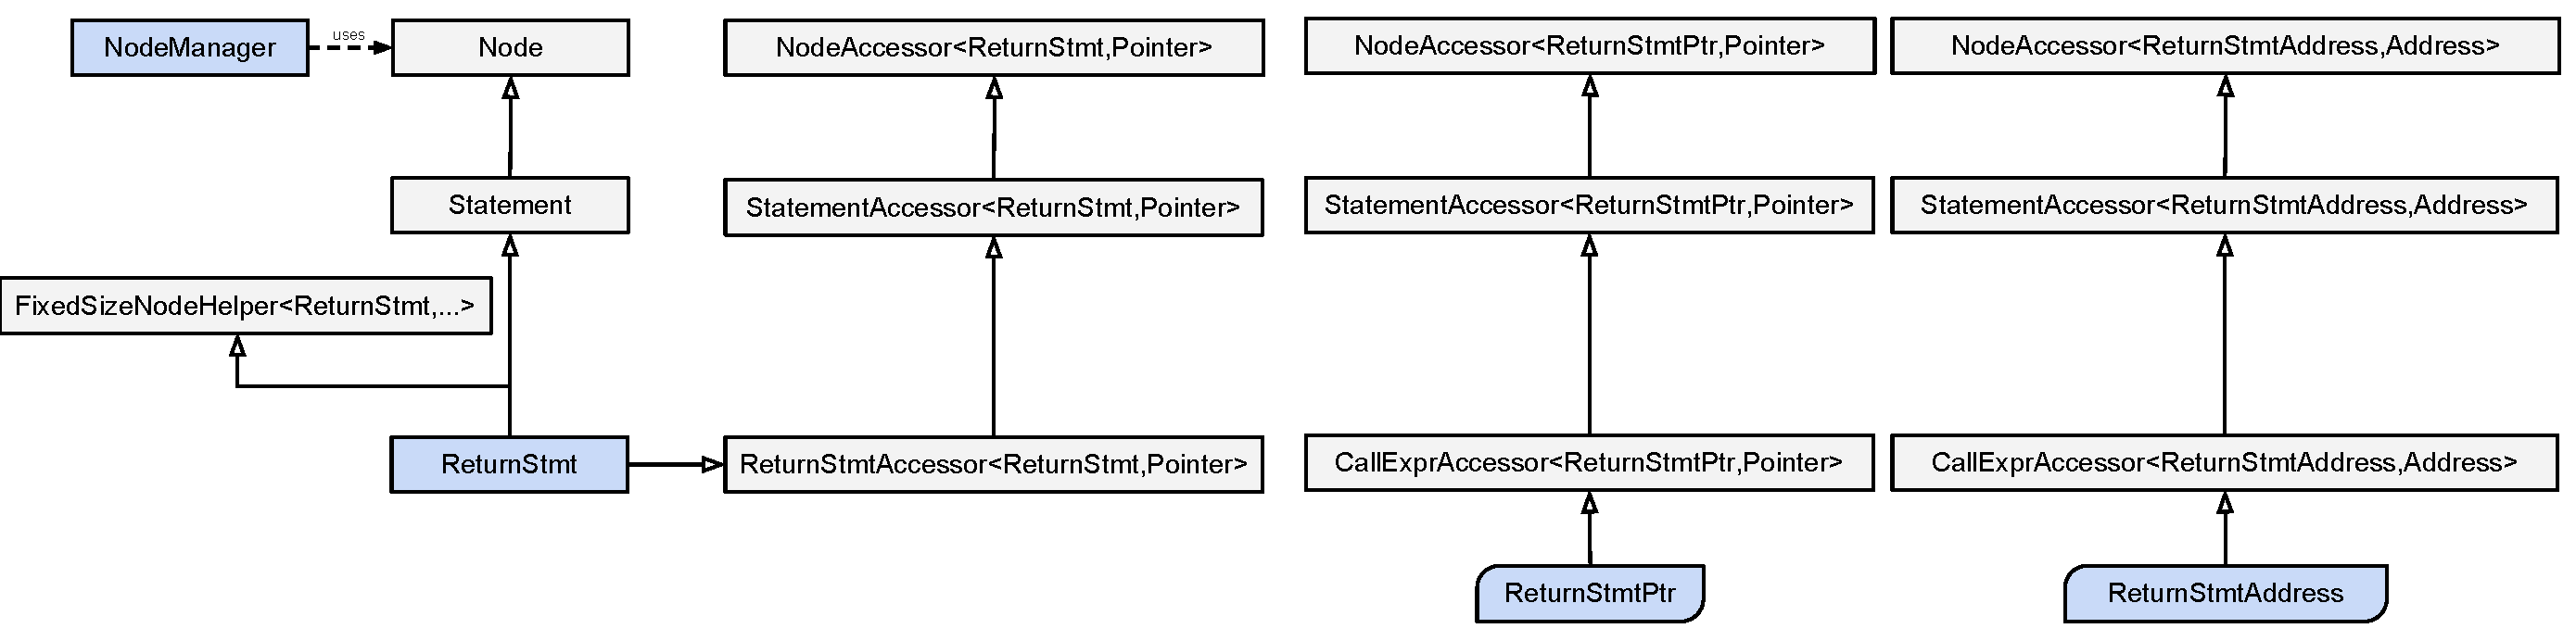
\includegraphics[width=\textwidth]{compiler/core/class_hierarchy_of_return_stmt.pdf}
	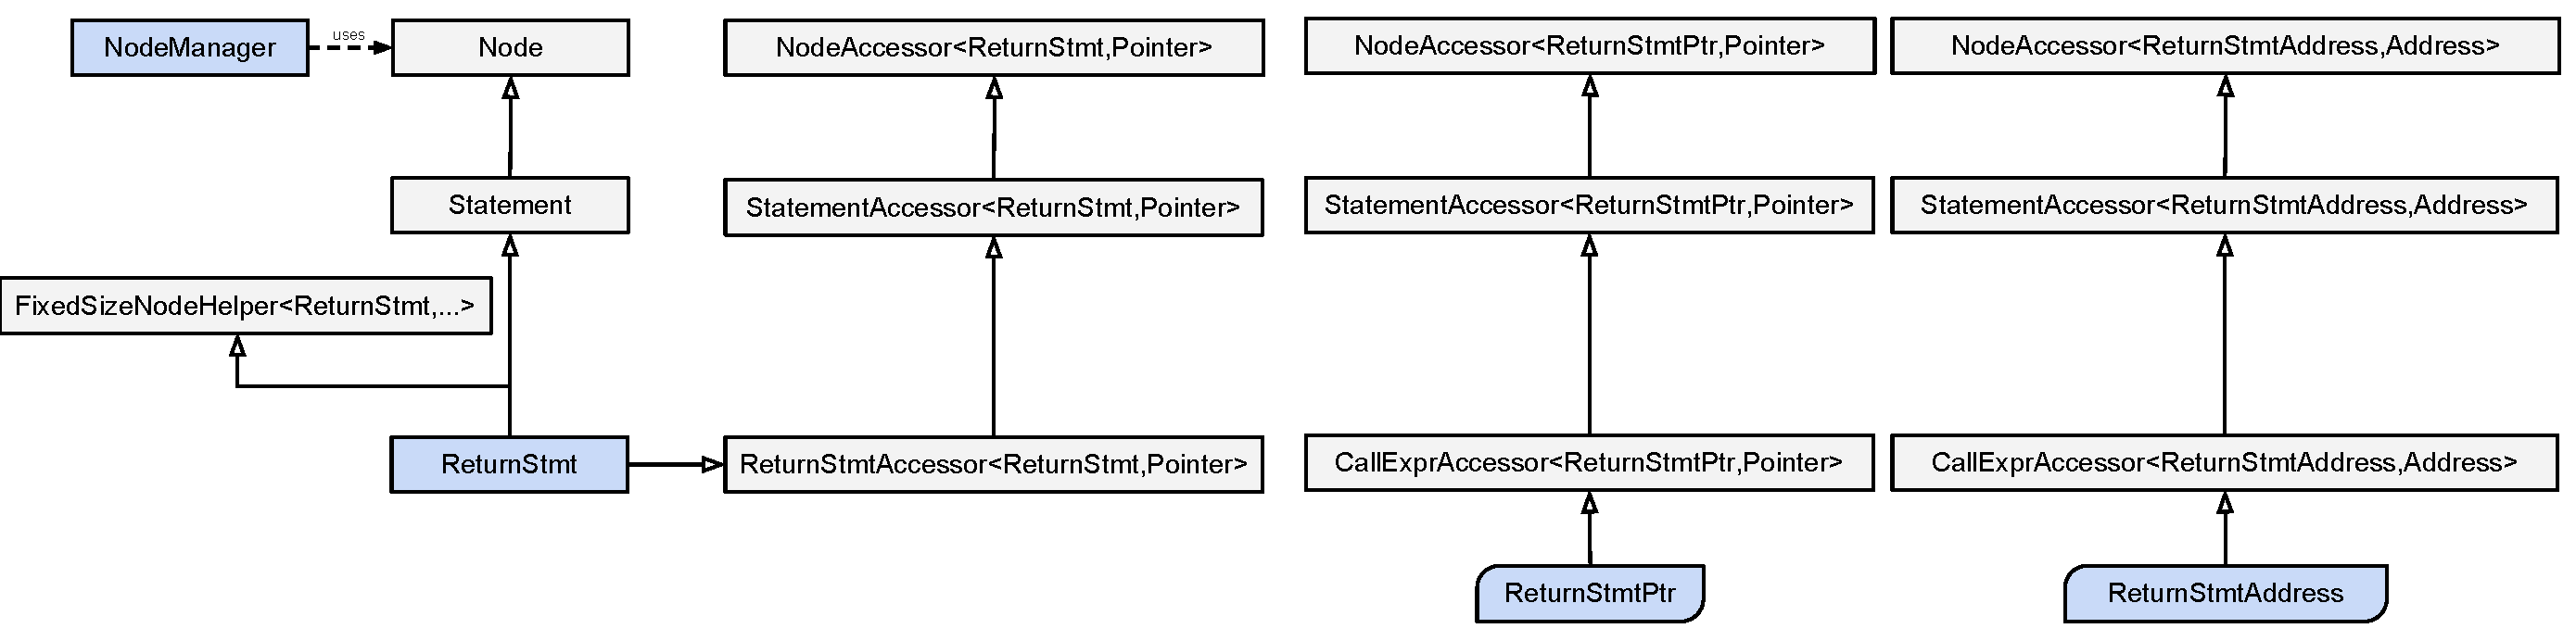
\includegraphics[width=\textwidth/4*3, trim=0 50 670 0, clip]{compiler/core/class_hierarchy_of_return_stmt.pdf}
	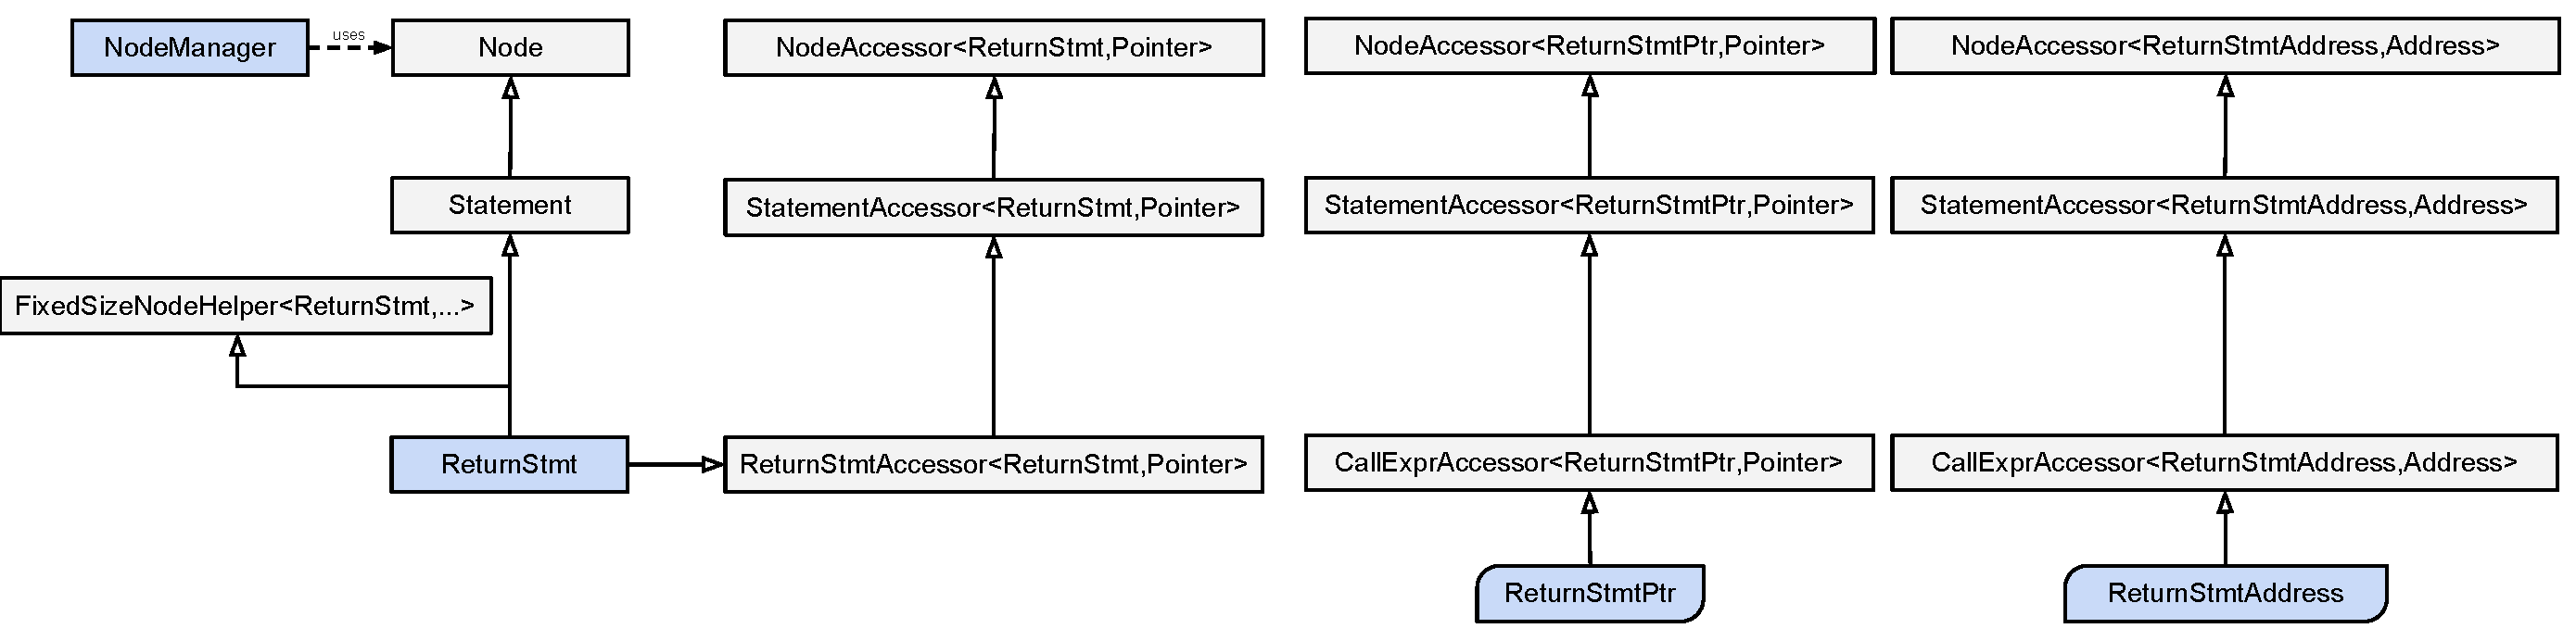
\includegraphics[width=\textwidth/4*3, trim=670 0 0 0, clip]{compiler/core/class_hierarchy_of_return_stmt.pdf}
	\caption{Relations between Classes contributing to the ReturnStmt}
	\label{fig:Compiler.Core.Classes.ReturnStmt}
\end{figure}
The blue boxes mark types being exposed to the user. The gray boxes are various
instantiations of generic types contributing the required functionality. The
following concrete classes are contributing to the architecture:
\begin{itemize}
  \item \type{Node} \ldots the generic base type
  \item \type{Statement} \ldots the common base type of all statements extending
  the node. This type inheritance allows Statements to be treated like any
  other Node.
  \item \type{ReturnStmt} \ldots the class implementing a return statement in
  the IR.
  IT is a extending the Statement type. It is only defining the type and a
  factory function (see code documentation), yet it does not define observer /
  getter methods.
  \item \type{NodeAccessor} \ldots a generic type defining all observer /
  getter methods applicable to nodes in general. The template is exploiting
  static dispatching for addressing requests to the actual instance derived from
  the generic base class. This way, overheads in memory requirements and
  execution time should be avoided. The second template parameter defines the
  reference type returned by involved getters. For more details on the
  parameters see the source code documentation \cite{insieme_source_doc}.
  \item \type{StatementAccessor} \ldots a generic accessor extending the basic
  NodeAccessor by all observer functions offered by any statement
  \item \type{ReturnStmtAccessor} \ldots a generic accessor extending the
  statement accessor by the extra functions offered by ReturnStmt nodes.
  \item \type{ReturnStmtPtr} \ldots the type of pointer used to reference
  ReturnStmt nodes. It uses the same hierarchy of generic types to obtain the required
  functionality as the node implementation itself does. However, it used
  different types to instantiate the offered generic parameters. Hence, every
  observer function only needs to be implemented once -- in a generic context.
  \item \type{ReturnStmtAddress} \ldots the address based counterpart of the
  ReturnStmtPtr
  \item \type{FixedSizeNodeHelper} \ldots a generic variadic template utility
  class implementing type save accesses to members of the child list -- which forms
  the foundation for all observer functions defined within the Accessors.
\end{itemize}


In the implementation two types of nodes are distinguished. The first, the
\type{FixedSizeNode} \index{IR!FixedSizeNode} type covers nodes having a fixed
size list of arbitrarily typed child nodes (like a tupel). For instance, the
ReturnStmt is a FixedSizeNode having a single child node -- the expression
computing the value to be returned. The second type is the \type{ListNode}
\index{IR!ListNode}.
In addition to a fixed set of child nodes, ListNodes may have a variable length list
of child nodes of a homogeneous type. An example is the \type{CallExpr}. It
child list has the shape
$$TypePtr, ExpressionPtr, ExpressionPtr^*$$
where the type is the type of the value represented by the call expression, the
first expression corresponds to the function to be called and the remaining
expressions to the arguments to be passed to the function. For \type{ListNodes}
the \lstinline|FixedSizeNodeHelper| is replaced by the \lstinline|ListNodeHelper|
and an additional layer of a \lstinline|ListNodeAccessor<>| class is introduced
at the bottom of the accessor hierarchy to support type-safe accesses to the
tailing node list. Figure \ref{fig:Compiler.Core.Classes.CallExpr} illustrates
the resulting class hierarchy of the \type{CallExpr}.
\begin{figure}[!tb]
	\centering
	%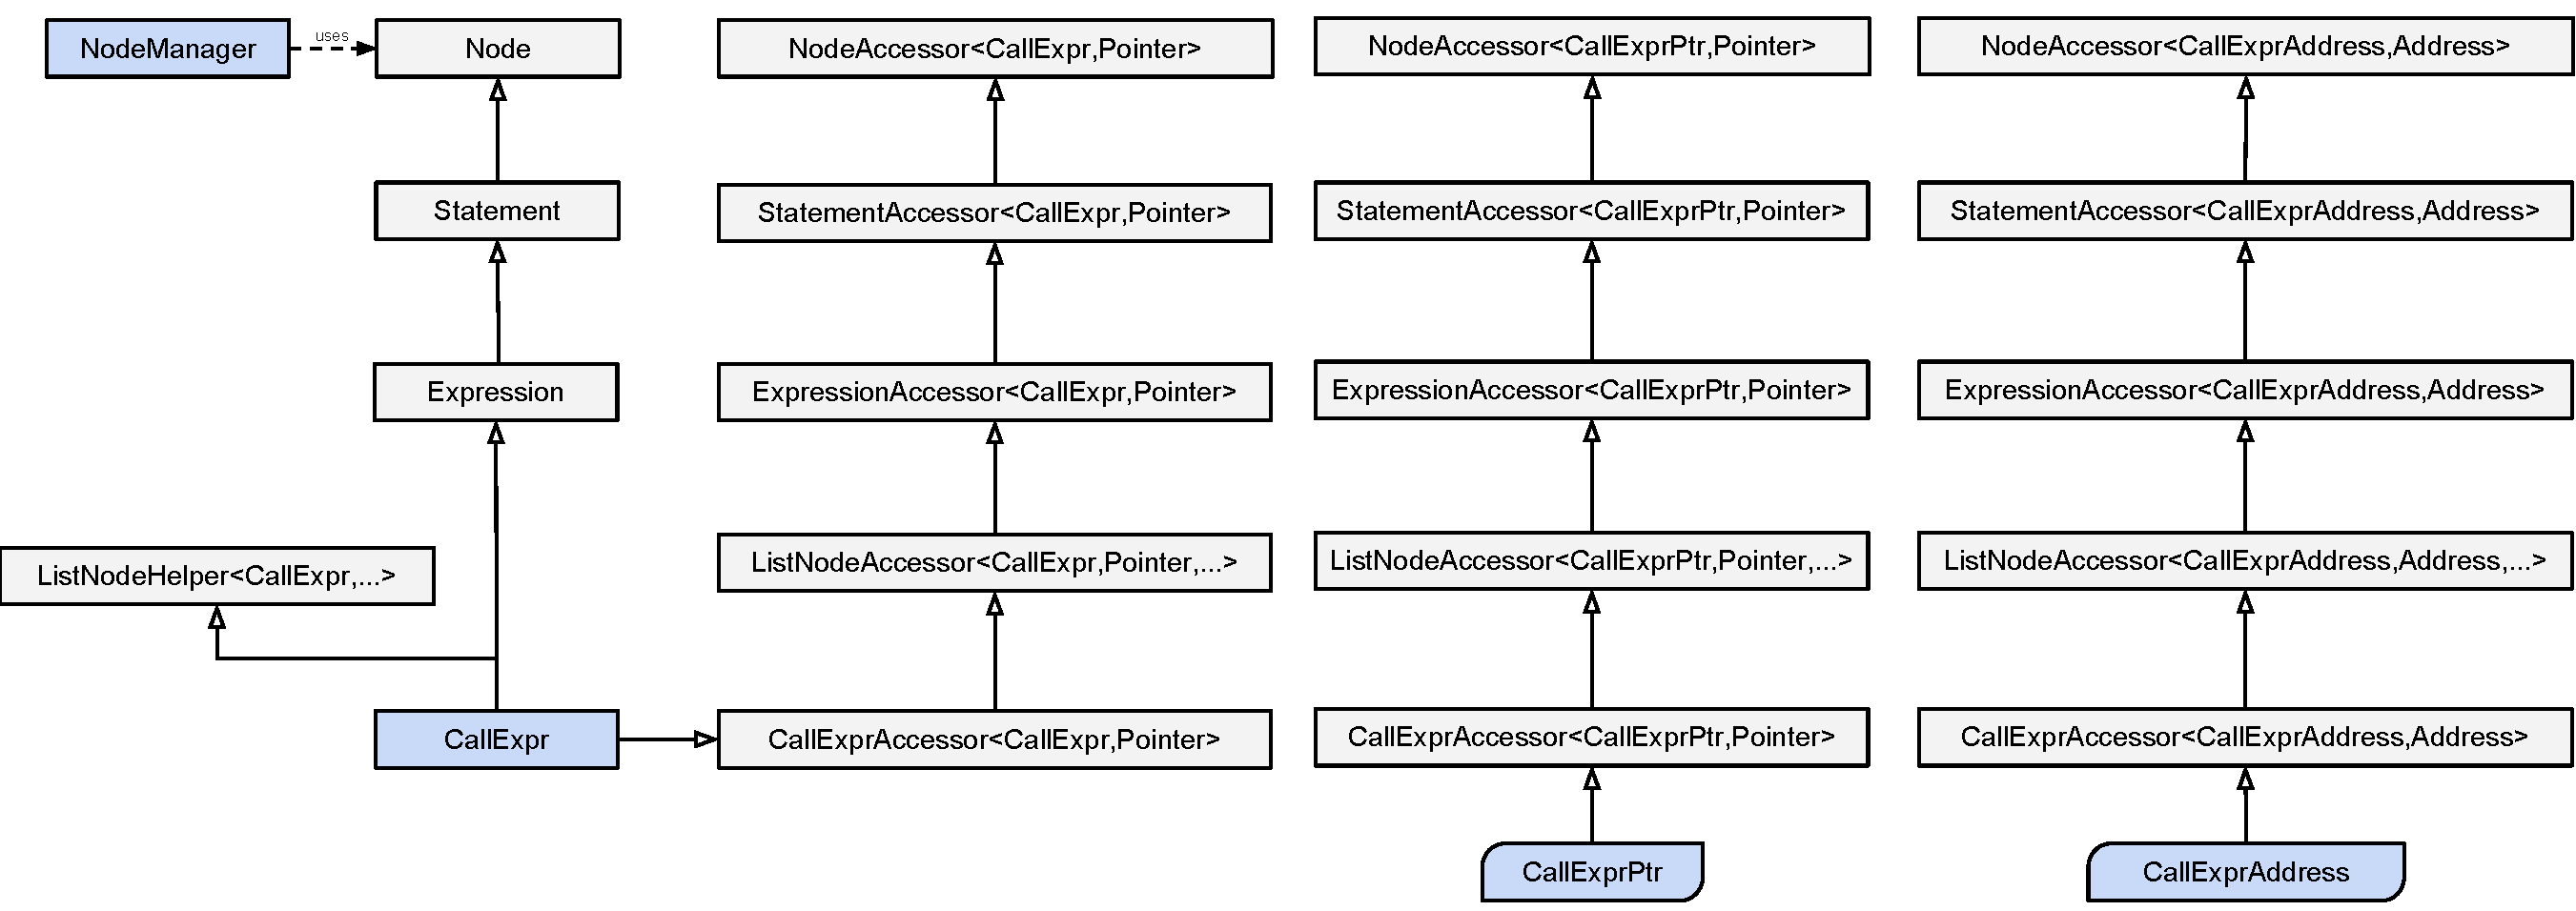
\includegraphics[width=\textwidth]{compiler/core/class_hierarchy_of_call_expr.pdf}
	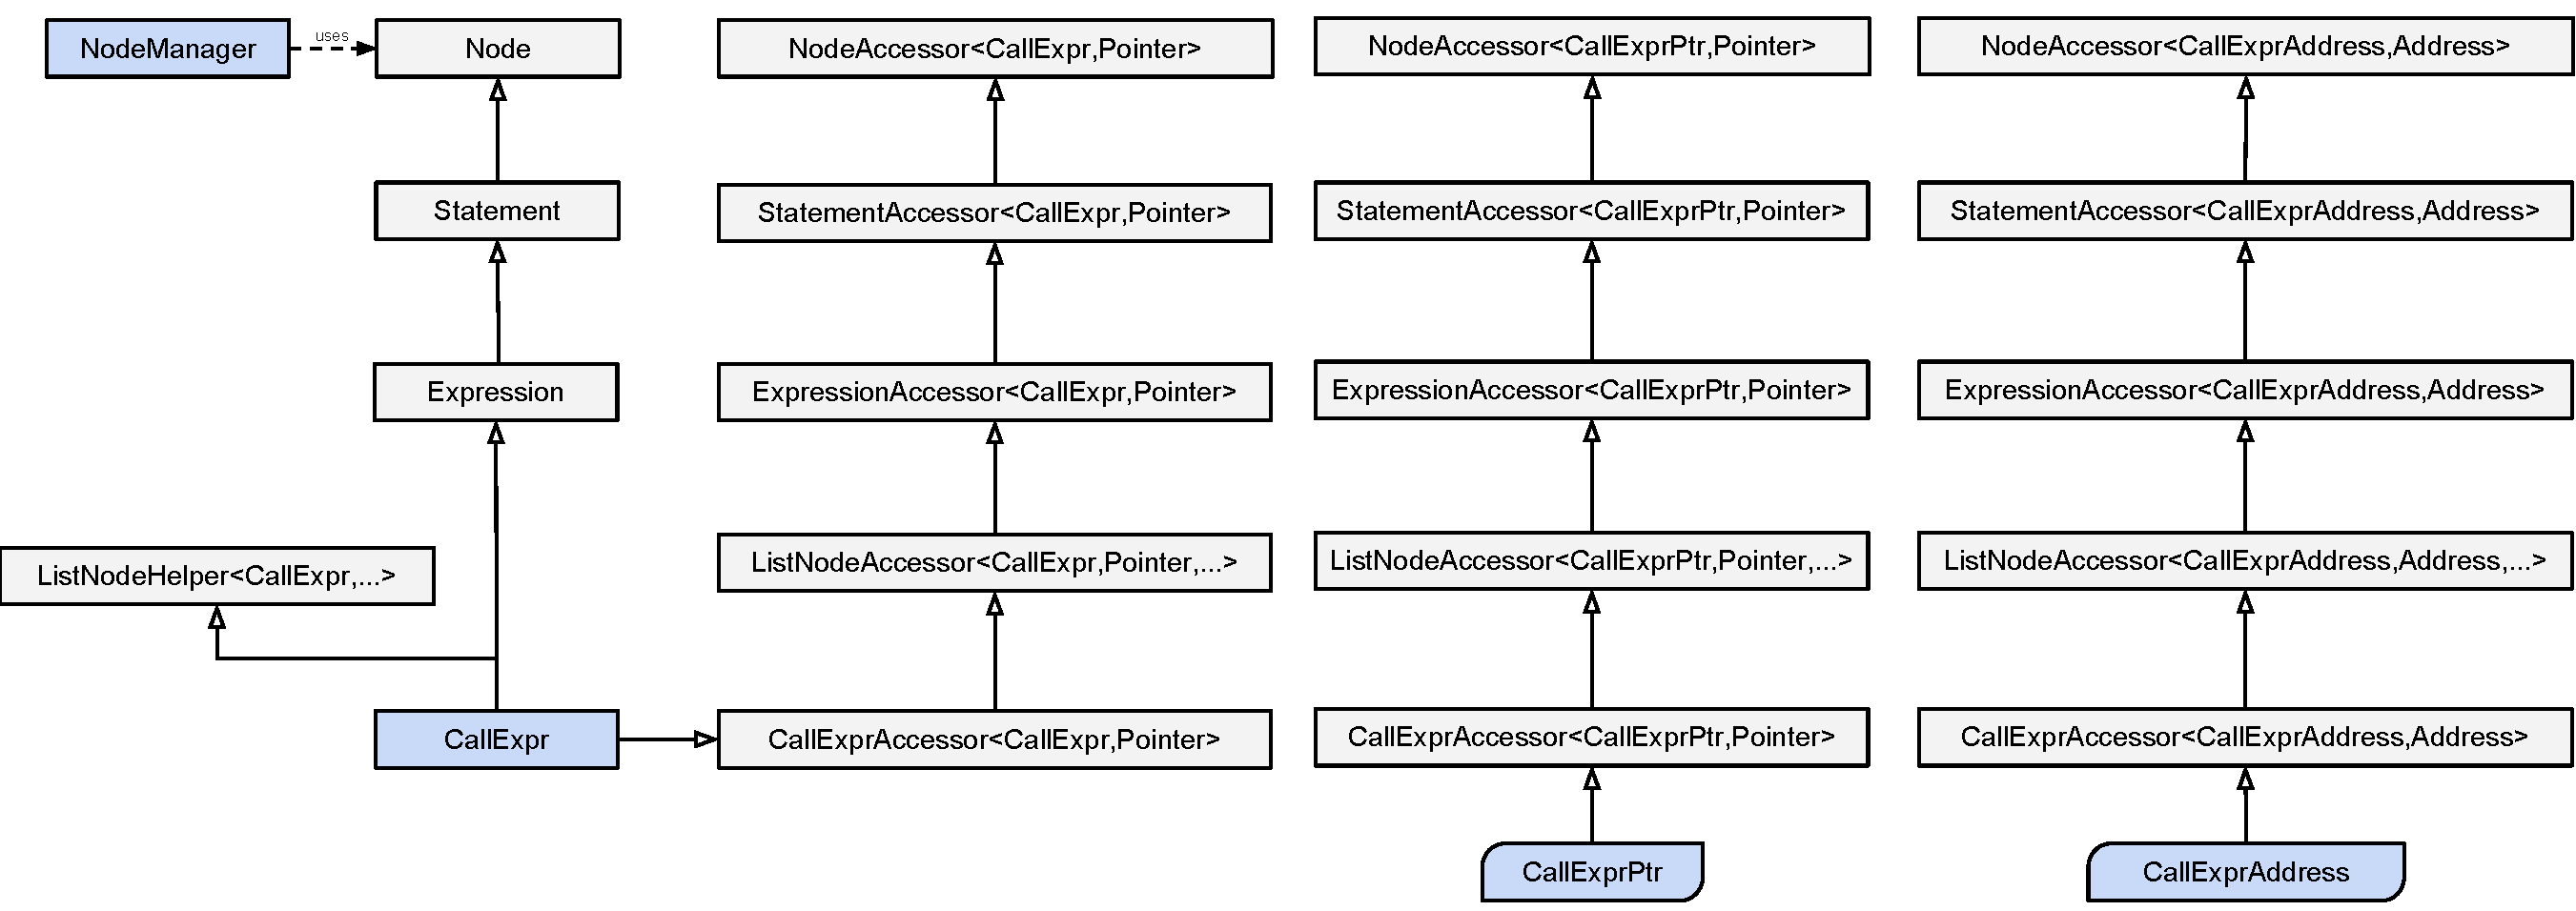
\includegraphics[width=\textwidth/4*3, trim=0 50 650 0, clip]{compiler/core/class_hierarchy_of_call_expr.pdf}
	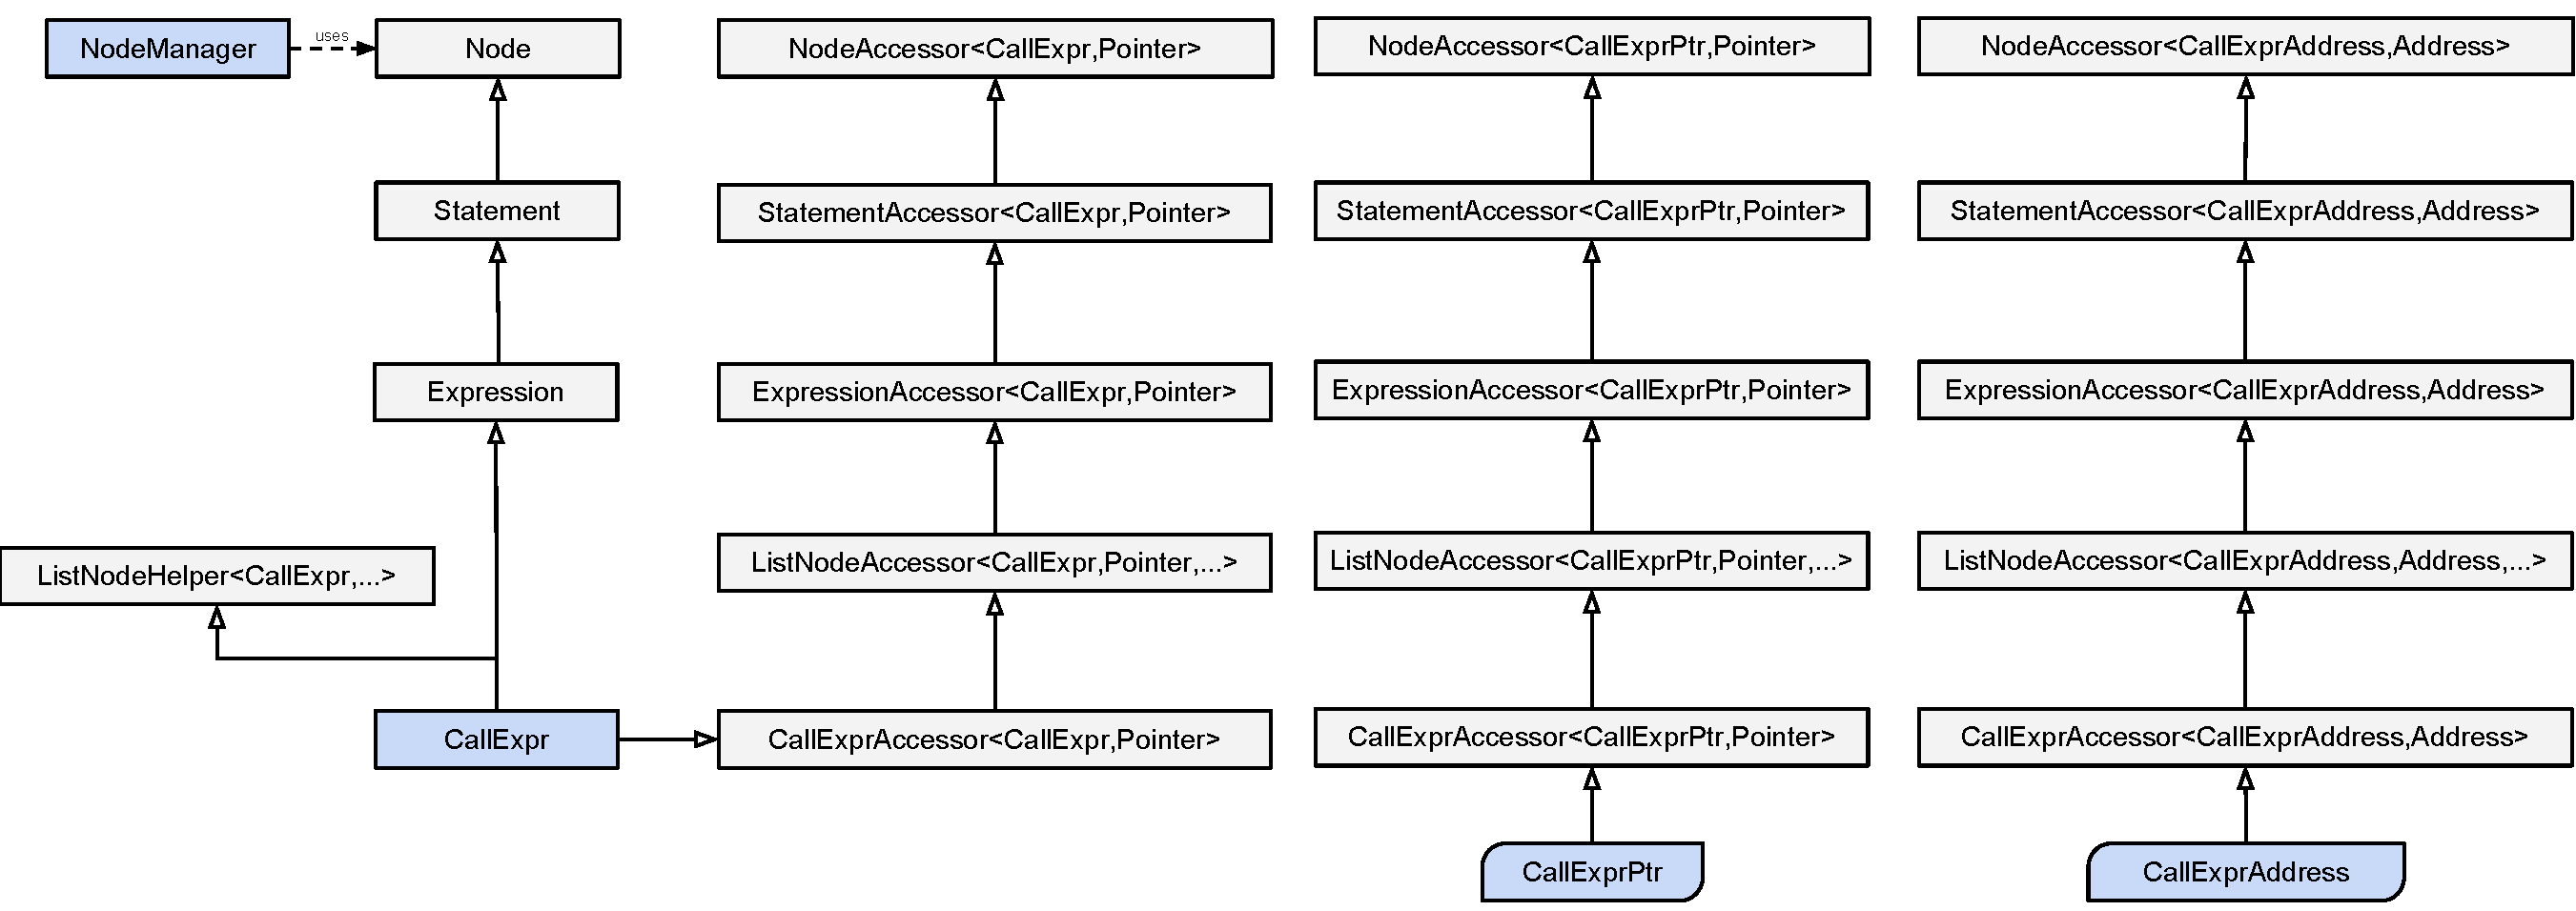
\includegraphics[width=\textwidth/4*3, trim=650 0 0 0, clip]{compiler/core/class_hierarchy_of_call_expr.pdf}
	\caption{Relations between Classes contributing to the CallExpr}
	\label{fig:Compiler.Core.Classes.CallExpr}
\end{figure}
Note: although the CallExprPtr type inherits from 5 classes it is not virtual.
It also just requires the size of a single pointer in memory and does not
introduce any overhead for construction / destruction except of setting the
pointer-member field. This light-weight property is especially desirable
when considering the fact that instances of NodePointers are created and
destroyed billions of times when running compiler code.

\subsubsection{Macros}
The restrictions imposed on nodes makes the implementation of the actual
instances a quite mechanical task -- and is therefore left to marcos. Within
\file{ir\_node.h} the following Macros are defined to generate node Accessors
and Node Implementations: 
\begin{itemize}
  \item IR\_NODE \ldots creates the head of a Node
  type definition including classes to be extended and a set of required constructors and a default
  factory. This Macro should be used to define new Node classes and extend those
  by static factory methods. 
  \item IR\_NODE\_ACCESSOR \ldots creates
  the head of a NodeAccessor definition for a FixedSizeNode including all
  dependencies and some member type definitions. The macro accepts a variable
  length argument list which has to be instantiated by the list of types
  expected to form the child list of the corresponding node.
  \item IR\_LIST\_NODE\_ACCESSOR \ldots the same as the IR\_NODE\_ACCESSOR
  macro, yet generating a NodeAccessor definition header for ListNodes.
\end{itemize}
However, those might only be used for creating
concrete nodes (nodes forming leafs of the type hierarchy, e.g. CallExpr), not
for abstract nodes within the type hierarchy (e.g. Statement, Expression,
\ldots). Those need to be implemented manually. For an extensive set of examples
on their application readers are referred to the existing node implementations.

\subsubsection{The NodeType Enumeration}
The X-macro file \file{ir\_nodes.def} defines the list of all existing node
types and their direct inheritance relation ship. It is used at various places
for statically generating codes depending on this information using the C
pre-processor. An example case is the definition of the NodeType enumeration
within \file{ir\_node\_types.h}. 

Every node instance is exposing its type via the \lstinline|getNodeType()|
method (defined within the generic NodeAccessor). This function can therefore be
used to determine the type of a node.


\subsubsection{Special Algorithms}
Within this subsection a view specific algorithms involved in the managing of
nodes will be discussed. 

\paragraph{Implicit Node Sharing} \index{IR!Node Sharing}
The virtual IR trees are internally maintained as a DAG by sharing identical
sub-trees. To realize this, a mean allowing to determine whether a certain node
instance already exists is required. This is among the central obligations
of the \type{NodeManager}s (beside the life-cycle management).

The InstanceManager, a generic utility class the \type{NodeManager} is based on, is
maintaining a set of all nodes currently ``alive'' within its domain. This set
is a hash based data structure. Therefore, every element within the set has to
offer a hash value and an equality function. Both requirements are satisfied by
the Node base class (which is possible do to the constraints defined by
\ref{eq:Compiler.Core.NodeDef}).

Whenever a Node is created, the following procedure is conducted:
\begin{enumerate}
  \item The Type and the Child-Node List is obtained (e.g. via an argument of
  the factory function)
  \item A local instance of the resulting node is created on the stack
  \item It is passed to the manager to obtain the ``master copy'' of
  requested node
  \item The manager computes the nodes hash value (by using one of its methods)
  to perform a look-up; the look-up first checks base-managers recursively (if
  chained) before checking the locally maintained set
  \item If present, the manager returns a reference to the obtained master copy
  \item If not present, a new master copy is created by cloning the handed in
  temporary node and a reference to the new node is returned
  \item The temporary copy on the stack is destroyed 
\end{enumerate}

In the concrete case of a ReturnStmt all those steps are conducted within one of
its factory functions using the following line of code:
\begin{lstlisting}
	return manager.get(ReturnStmt(expression));
\end{lstlisting}

In the end, although the mechanism beneath is complex, the interface to the user
is kept as simple as possible. The node-sharing happens automatically.

\paragraph{Hashing} \index{IR!Hashing}
The hashing of Nodes is implemented within the static member function
\lstinline|hashNodes| of the Node class and the \lstinline|hash| functions
within the \file{ir\_node.cpp}. All of them are simply combining the hash
values of the child nodes with the NodeType using a boost utility function to
obtain a proper hash code. Therefore, the hash value of a node recursively
covers the entire virtual sub-tree rooted by the given node.

Since hashes are depending on the entire sub-tree, computing those can become
expensive. In fact, the recursive computation grows exponential with the height
of the IR tree. Fortunately, all nodes are immutable. Therefore, hashes can be
cached and computed once during construction -- by only accessing the already
cached hash codes of the child nodes. This way, the computation of the hash is
reduced to a local operation, hence $\mathcal{O}(1)$;

\paragraph{Equality} \index{IR!Equality Classes} 
For the look-up in the HashSet Nodes need to be tested for equality. If two
nodes are equivalent, this is quite easy. With a probability bordering on
certainty their hash values will be different. If not, node types or the
immediate child nodes are likely to be different. Hence, inequality can be
quickly (almost always locally) decided.

However, in case two nodes (and hence the represented sub-trees) are equivalent,
this cannot be decided as effectively with the provided means. Just because hash
values are identical does not allow to conclude that the corresponding trees are
equal. To make sure two trees are identical, every node within one tree has to
be compared to every node within the other tree. Hence, deciding whether two
trees are equivalent is an expensive operation -- considering the fact that
trees may consist of more than 10 million (virtual) nodes for moderate sized
codes.

To fix this problem, equivalence classes of nodes identified by simple integer
IDs are formed dynamically to cache comparison results. The mechanism is
implemented by the == operator of the Node class. Each node is created using an
equality class ID of 0 (hence, no class fixed yet). If it is ever compared to
another node and determined to be equivalent, the equality ID of the other node
is copied. If the other ID is also 0, a fresh equality ID is assigned to both
nodes. Future comparisons start by comparing the equality ID.
If both are not 0 and equal it can be immediately deduced that nodes are equal. If both are
not 0 and distinct, the comparison has to be continued recursively (they still
might be equal, just their equality classes never ``met'' so far). Finally, in
case two nodes are determined to be equivalent although their equality ID is set
and distinct, the larger equality ID will be replaced by the smaller one. This
way, equality classes are merging over time.

The locally stored integer allows to determine equality effectively using
locally available information. Even in the cases the local nodes does not have a
set equality ID, it is likely the child nodes have. Amortised, this should
result in a complexity of $\mathcal{O}(1)$ for determining whether two IR trees
are structurally identical.


  

\subsubsection{HowTo}
Finally, to conclude the documentation of the Node implementation some example
of common steps should be documented:

 \paragraph{Add a new Node} When ever adding a step, follow the following
 procedure:
 
\begin{enumerate}
  \item Do you really need a new node type or would a type, function or
  combination of existing nodes be sufficient?
  
  \item So, you're serious, you really need a new one? If not, just stop here.
  
  \item Register the new Node within the type hierarchy within
  \file{ir\_nodes.def}. This will automatically create an entry in the
  NodeType enumeration, add support within visitors, IR statistics and printers.
  
  \item Determine whether your new node is a FixedSizeNode or a ListNode.
  
  \item Pick a file to implement your new node. In the header file you have to
  define the accessor and the node class itself. Use the corresponding macros
  defined within \file{ir\_node.h}. When defining the accessor, fix the list
  of child node types.
  
  \item Add a list of accessor functions to the accessor using the
  IR\_NODE\_PROPERTY macro. Each macro is mapping a type and name to a certain
  location within the child-node list.

  \item If necessary you can add derived accessors (accessing nodes of
  child-nodes). For examples see the implementation of the ForStmtAccessor.
  
  \item Add required factory functions to the body of the node class definition.
  
  \item Rerun the cmake-script to trigger the IR builder generator (see
  \ref{sec:Compiler.Core.Builder} for details)
  
  \item Test your new node. You may extend one of the existing test cases.
  Essentially, would should be at least (!) done is to create an instance -- or
  more if complex combination of child lists are possible -- and run the
  \lstinline|basicNodeTests| implemented within \file{ir\_node\_test.inc}
  located in the test folder of the core project.
\end{enumerate}
 
 
\paragraph{Add a Member Field to a Node Type}
To add a new property to a node, process the following steps:
\begin{enumerate}
  \item Determine whether the new field requires a new entry in the child-list
  or whether it is a derived one.
  
  \item If derived: use the examples included within the ForStmt
  (for deriving nodes) or the LambdaExpr (for derived non-node
  values) implementations as an example
  
  \item If a new filed:
	\begin{itemize}
	  \item add the type of the new field to the child-type list
  	  within the corresponding NodeAccessor
  	  
  	  \item add a access method using the IR\_NODE\_PROPERTY macro

  	  \item if the new child node has not been appended to the end, fix the
  	  indexes of the remaining methods

  	  \item update the factory function, which will update the builder when
  	  running cmake the next time

  	  \item fix all depending utilities like the pretty printer, the backend or
  	  any code using the factory function (if not backward compatible)
	\end{itemize}
  
  \item Extend the existing test cases to cover the new node
\end{enumerate}

\paragraph{Add a Method to a Node Type} 
To add new method to a node, you should first think whether your desired
operation is of general interest -- hence, whether it has a wide enough
relevance to justify adding it to the node itself instead of realizing it
as a function within some external utility header. The node implementation
should be kept clean of use-case specific codes.

If you decide that your method is important / useful / convenient enough, you
should add it using the same procedure as has been described for derived members
within the previous HowTo. As an example you can have a look at the
\lstinline|isRecursive()| method of the \lstinline|LambdaExpr| node.


\paragraph{Migrate Codes between Node Managers}
When working with multiple node managers frequently the question regarding how
to migrate an IR DAG from one node manager to another. The answer is simple:
just ask the target manager for a reference to the corresponding IR structure.

For instance, let \lstinline|code| be a reference (NodePtr) to the root of some
IR structure. Let \lstinline|targetMgr| be the manager you want to obtain a copy
from it. Simply use 
\begin{lstlisting}
	auto copy = targetMgr.get(code);
\end{lstlisting}
to obtain the corresponding copy within the target manager. If your
\lstinline|nodeAddr| is of type \lstinline|NodeAddress| (or any other node
address) you can use 
\begin{lstlisting}
	auto copy = nodeAddr.cloneTo(targetMgr);
\end{lstlisting}
to obtain a lone of the address within the given target manager. Unlike the
pointer variant, this does not only clone the addressed node to the target
manager but also all the nodes along the path described by the address,
in particular including the root node.

\paragraph{Use Node Managers to form Local Scopes}
When entering a code section performing a heavy node manipulations,
hence generating a large number of temporary nodes it is recommended to use some
local manager to limit the life-cycles of temporary nodes. This mechanism can be
considered as some simple mechanism of garbage collection.

The following code example demonstrates how to use \type{NodeManager} chaining:
\begin{lstlisting}
	NodePtr process(const NodePtr& input) {
		// get reference to outer node manager
		NodeManager& outer = input->getNodeManager();
		// create local node manager
		NodeManager local(outer);
		// work with local manager
		NodePtr res = doSomething(input, local);
		// return result - ATTENTION: within the right node manager
		return outer.get(res);
	}
\end{lstlisting}
Some functions do not allow to pass a \type{NodeManager} as an argument. For those,
chained managers can not help to contain temporary node instances since they are
using the \type{NodeManager} managing the input node. Note, passing
\lstinline|local.get(input)| as an argument does not help, since it is just the
same as passing \lstinline|input| (inherited from the outer \type{NodeManager}).

In the core, most operations offer the possibility to pass the \type{NodeManager} to be
used as an argument. Otherwise, to isolated the creation of temporary nodes, an
independent \type{NodeManager} instance can be used as follows:
\begin{lstlisting}
	NodePtr process(const NodePtr& input) {
		// get reference to outer node manager
		NodeManager& outer = input->getNodeManager();
		// create local node manager
		NodeManager local;
		// work with local manager
		NodePtr res = doSomething(local.get(input);
		// return result - ATTENTION: within the right node manager
		return outer.get(res);
	}
\end{lstlisting}
However, in this case all nodes referenced (transitively) by the input node will
have to be copied to the new node manager. On the other hand, the total
isolation even enables to work on the various copies in parallel, as will be
covered within the following section.

\paragraph{Use multiple Node Managers in Parallel Contexts}
Although generally immutable, the managing of nodes within the manager and the
handling of annotations is not synchronized. \note{This is something which
really should be fixed in the future!} Therefore, when operating on IRs in
parallel including the creation of nodes, each thread has to work on its own
copy using a local (private) non-chained node manager. 

Therefore, just create a local \type{NodeManager} and clone the IR to be processed to
your local manager. Further on you can run your operations in parallel on the
individual clones. Attention: if you want to return a value, you have to copy
the result back into the original \type{NodeManager} -- which should happen in a
synchronized way.

Some operations operating on IR nodes require the generation of fresh IDs (e.g.
variable IDs). Those IDs are managed by the \type{NodeManager}. After creating a local
manager, the next ID will be 1 again -- since none has been assigned yet.
Further, cloning IR structures into the manager will not change this
circumstance. In rare cases it can happen this way that presumably unique IDs
are used for new nodes which further on produce collisions since the same IDs
have been used before.\note{This is also something which should be fixed
soon. (I bet this note will be here forever)}

To prevent this from happening, after creating your private \type{NodeManager} the
fresh-value ID should be seeded. This can be conducted using the following code
snippet (also includes the parallel node manager creation):
\begin{lstlisting}
	core::StatementAddress trg = someSource(...);
	
	#pragma omp parallel
	{
		core::NodeManager local;
		core::StatementAddress localTargetCopy;

		#pragma omp critical
		{
			local.setNextFreshID(trg->getNodeManager().getFreshID());
			localTargetCopy = trg.cloneTo(local);
		}
	
		// run parallel operations

	}
	// temporaries automatically cleaned up
\end{lstlisting}


\begin{comment}
The main obligation of the core is to provide the data structures to model 

Sections:
\begin{itemize}
  \item General idea of the DAG and the sharing
  \item Involved classes and files and their relationship
  \item Implementation details of the classes
  \item The various node types
  \item Special Algorithms - hashing, equality
  \item HOW-TOs
\end{itemize}


To be covered:
\begin{itemize}
  \item Purpose of Nodes - distinction to the IR Spec
  \item Fact that nodes form a DAG
  \item Node Identity specified by type + children or value (little formally)
  \item Node Manager concept for memory management and sharing
  \item Handling the node manager in parallel environments
  \item Implementation of nodes (macros and generics)
  \item List of involved files (nodes.def, ir\_nodes.h, ir\_types.h)
  \item NodeType, NodeCategory, Nodes, Values, Types, Expressions, Statements,
  Support, Program, Accessors, \ldots + relations
  \item How to add new nodes
  \item How to add a method to a node
  \item How to add a field to a node (when to do so - e.g. not if it is
  something identity critical)
  \item Hashing and equality determination.
\end{itemize}

\subsubsection{Types}
\subsubsection{Statements}
\subsubsection{Expressions}
\subsubsection{Support}
\end{comment}
